\documentclass{article}
\usepackage[paperwidth=6.5in,paperheight=2in,margin=0in]{geometry}
\usepackage{mathptmx}%{times}
\usepackage{graphicx}
\usepackage{siunitx}
\usepackage[absolute,overlay]{textpos}
\usepackage{color}

\setlength{\parindent}{0pt}
\begin{document}
\TPMargin{1pt}
\begin{textblock}{4}(2.5,0)
\normalsize
(a) $t=\SI{0}{\second}$
\end{textblock}
\begin{textblock}{4}(7.5,0)
\normalsize
(b) $t=T/2$
\end{textblock}
\begin{textblock}{4}(12.5,0)
\normalsize
(c) $t=T$
\end{textblock}
\vspace*{0.4em}
\includegraphics{../deformationSphere-gaussians-nondiv-cubicUpwind-hex-8/0/tracer.pdf}
\hspace*{0.2em}
\includegraphics{../deformationSphere-gaussians-nondiv-cubicUpwind-hex-8/518400/tracerW.pdf}
\hspace*{0.2em}
\includegraphics{../deformationSphere-gaussians-nondiv-cubicUpwind-hex-8/1.0368e+06/tracerW.pdf} \\
\centering
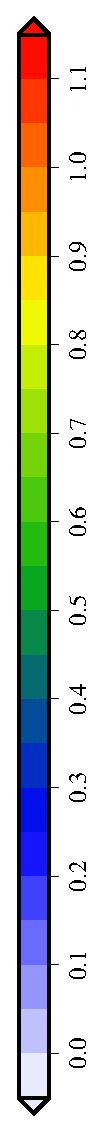
\includegraphics[height=5in,angle=270]{deformationSphere-T-legend.eps}
\end{document}
